% This is the Reed College LaTeX thesis template. Most of the work
% for the document class was done by Sam Noble (SN), as well as this
% template. Later comments etc. by Ben Salzberg (BTS). Additional
% restructuring and APA support by Jess Youngberg (JY).
% Your comments and suggestions are more than welcome; please email
% them to cus@reed.edu
%
% See https://www.reed.edu/cis/help/LaTeX/index.html for help. There are a
% great bunch of help pages there, with notes on
% getting started, bibtex, etc. Go there and read it if you're not
% already familiar with LaTeX.
%
% Any line that starts with a percent symbol is a comment.
% They won't show up in the document, and are useful for notes
% to yourself and explaining commands.
% Commenting also removes a line from the document;
% very handy for troubleshooting problems. -BTS

% As far as I know, this follows the requirements laid out in
% the 2002-2003 Senior Handbook. Ask a librarian to check the
% document before binding. -SN

%%
%% Preamble
%%
% \documentclass{<something>} must begin each LaTeX document
\documentclass[12pt,twoside]{templates/facsothesis}
% Packages are extensions to the basic LaTeX functions. Whatever you
% want to typeset, there is probably a package out there for it.
% Chemistry (chemtex), screenplays, you name it.
% Check out CTAN to see: https://www.ctan.org/
%%
\ifxetex
  \usepackage{polyglossia}
  \setmainlanguage{spanish}
  % Tabla en lugar de cuadro
  \gappto\captionsspanish{\renewcommand{\tablename}{Tabla}
          \renewcommand{\listtablename}{Índice de tablas}}
\else
  \usepackage[spanish,es-tabla]{babel}
\fi
%\usepackage[spanish]{babel}
\usepackage{graphicx,latexsym}
\usepackage{amsmath}
\usepackage{amssymb,amsthm}
\usepackage{longtable,booktabs,setspace}
\usepackage{chemarr} %% Useful for one reaction arrow, useless if you're not a chem major
\usepackage[hyphens]{url}
% Added by CII
%\usepackage{hyperref}
\usepackage[colorlinks = true,
            linkcolor = blue,
            urlcolor  = blue,
            citecolor = blue,
            anchorcolor = blue]{hyperref}
\usepackage{lmodern}
\usepackage{float}
\floatplacement{figure}{H}
% End of CII addition
\usepackage{rotating}
\usepackage{placeins} % para fijar la posición de las tablas con \FloatBarrier


\usepackage[]{natbib}


% Next line commented out by CII
%\usepackage{biblatex}
%\usepackage{natbib}
% Comment out the natbib line above and uncomment the following two lines to use the new
% biblatex-chicago style, for Chicago A. Also make some changes at the end where the
% bibliography is included.
%\usepackage{biblatex-chicago}
%\bibliography{thesis}


% Added by CII (Thanks, Hadley!)
% Use ref for internal links
\renewcommand{\hyperref}[2][???]{\autoref{#1}}
\def\chapterautorefname{Chapter}
\def\sectionautorefname{Section}
\def\subsectionautorefname{Subsection}
% End of CII addition

% Added by CII
\usepackage{caption}
\captionsetup{width=5in}
% End of CII addition

% \usepackage{times} % other fonts are available like times, bookman, charter, palatino

% Syntax highlighting #22
  \usepackage{color}
  \usepackage{fancyvrb}
  \newcommand{\VerbBar}{|}
  \newcommand{\VERB}{\Verb[commandchars=\\\{\}]}
  \DefineVerbatimEnvironment{Highlighting}{Verbatim}{commandchars=\\\{\}}
  % Add ',fontsize=\small' for more characters per line
  \usepackage{framed}
  \definecolor{shadecolor}{RGB}{248,248,248}
  \newenvironment{Shaded}{\begin{snugshade}}{\end{snugshade}}
  \newcommand{\AlertTok}[1]{\textcolor[rgb]{0.94,0.16,0.16}{#1}}
  \newcommand{\AnnotationTok}[1]{\textcolor[rgb]{0.56,0.35,0.01}{\textbf{\textit{#1}}}}
  \newcommand{\AttributeTok}[1]{\textcolor[rgb]{0.77,0.63,0.00}{#1}}
  \newcommand{\BaseNTok}[1]{\textcolor[rgb]{0.00,0.00,0.81}{#1}}
  \newcommand{\BuiltInTok}[1]{#1}
  \newcommand{\CharTok}[1]{\textcolor[rgb]{0.31,0.60,0.02}{#1}}
  \newcommand{\CommentTok}[1]{\textcolor[rgb]{0.56,0.35,0.01}{\textit{#1}}}
  \newcommand{\CommentVarTok}[1]{\textcolor[rgb]{0.56,0.35,0.01}{\textbf{\textit{#1}}}}
  \newcommand{\ConstantTok}[1]{\textcolor[rgb]{0.00,0.00,0.00}{#1}}
  \newcommand{\ControlFlowTok}[1]{\textcolor[rgb]{0.13,0.29,0.53}{\textbf{#1}}}
  \newcommand{\DataTypeTok}[1]{\textcolor[rgb]{0.13,0.29,0.53}{#1}}
  \newcommand{\DecValTok}[1]{\textcolor[rgb]{0.00,0.00,0.81}{#1}}
  \newcommand{\DocumentationTok}[1]{\textcolor[rgb]{0.56,0.35,0.01}{\textbf{\textit{#1}}}}
  \newcommand{\ErrorTok}[1]{\textcolor[rgb]{0.64,0.00,0.00}{\textbf{#1}}}
  \newcommand{\ExtensionTok}[1]{#1}
  \newcommand{\FloatTok}[1]{\textcolor[rgb]{0.00,0.00,0.81}{#1}}
  \newcommand{\FunctionTok}[1]{\textcolor[rgb]{0.00,0.00,0.00}{#1}}
  \newcommand{\ImportTok}[1]{#1}
  \newcommand{\InformationTok}[1]{\textcolor[rgb]{0.56,0.35,0.01}{\textbf{\textit{#1}}}}
  \newcommand{\KeywordTok}[1]{\textcolor[rgb]{0.13,0.29,0.53}{\textbf{#1}}}
  \newcommand{\NormalTok}[1]{#1}
  \newcommand{\OperatorTok}[1]{\textcolor[rgb]{0.81,0.36,0.00}{\textbf{#1}}}
  \newcommand{\OtherTok}[1]{\textcolor[rgb]{0.56,0.35,0.01}{#1}}
  \newcommand{\PreprocessorTok}[1]{\textcolor[rgb]{0.56,0.35,0.01}{\textit{#1}}}
  \newcommand{\RegionMarkerTok}[1]{#1}
  \newcommand{\SpecialCharTok}[1]{\textcolor[rgb]{0.00,0.00,0.00}{#1}}
  \newcommand{\SpecialStringTok}[1]{\textcolor[rgb]{0.31,0.60,0.02}{#1}}
  \newcommand{\StringTok}[1]{\textcolor[rgb]{0.31,0.60,0.02}{#1}}
  \newcommand{\VariableTok}[1]{\textcolor[rgb]{0.00,0.00,0.00}{#1}}
  \newcommand{\VerbatimStringTok}[1]{\textcolor[rgb]{0.31,0.60,0.02}{#1}}
  \newcommand{\WarningTok}[1]{\textcolor[rgb]{0.56,0.35,0.01}{\textbf{\textit{#1}}}}

% To pass between YAML and LaTeX the dollar signs are added by CII
\title{Título completo de la tesis o seminario de grado}
\author{Mi nombre}
% The month and year that you submit your FINAL draft TO THE LIBRARY (May or December)
\date{Fecha}
\division{}
\advisor{Profesor/a guía: mi supervisor/a}
\institution{Universidad de Chile}
\degree{Seminario / Memoria / Tesis de Grado - Carrera de Sociología}
%If you have two advisors for some reason, you can use the following
% Uncommented out by CII
% End of CII addition

%%% Remember to use the correct department!
\department{}
% if you're writing a thesis in an interdisciplinary major,
% uncomment the line below and change the text as appropriate.
% check the Senior Handbook if unsure.
%\thedivisionof{The Established Interdisciplinary Committee for}
% if you want the approval page to say "Approved for the Committee",
% uncomment the next line
%\approvedforthe{Committee}

% Added by CII
%%% Copied from knitr
%% maxwidth is the original width if it's less than linewidth
%% otherwise use linewidth (to make sure the graphics do not exceed the margin)
\makeatletter
\def\maxwidth{ %
  \ifdim\Gin@nat@width>\linewidth
    \linewidth
  \else
    \Gin@nat@width
  \fi
}
\makeatother

%Added by @MyKo101, code provided by @GerbrichFerdinands

\setlength\parindent{0pt}


% Added by CII

\providecommand{\tightlist}{%
  \setlength{\itemsep}{0pt}\setlength{\parskip}{0pt}}

\Acknowledgements{

}

\Dedication{

}

\Preface{

}

\Abstract{

}

% End of CII addition
%%
%% End Preamble
%%
%
\let\chaptername\relax
\begin{document}
\bibliographystyle{apalike}
% Everything below added by CII
  \maketitle

\frontmatter % this stuff will be roman-numbered
\pagestyle{empty} % this removes page numbers from the frontmatter



%  \hypersetup{linkcolor=black}
  \setcounter{tocdepth}{1}
  \setlength{\parskip}{0pt}
  \tableofcontents

\setlength\parskip{1em plus 0.1em minus 0.2em}

  \listoftables

  \listoffigures



\mainmatter % here the regular arabic numbering starts
\pagestyle{fancyplain} % turns page numbering back on

\hypertarget{resumen}{%
\chapter*{Resumen}\label{resumen}}
\addcontentsline{toc}{chapter}{Resumen}

Resumen aquí

\hypertarget{agradecimientos}{%
\chapter*{Agradecimientos}\label{agradecimientos}}
\addcontentsline{toc}{chapter}{Agradecimientos}

Agradecimientos aquí.

\hypertarget{introducciuxf3n-tesisfacsodown}{%
\chapter{Introducción: tesisfacsodown}\label{introducciuxf3n-tesisfacsodown}}

Tesisfacsodown es básicamente una propuesta o plantilla para poder escribir un trabajo final formateado en alta calidad, con opción tanto para pdf como para html. Para ello, basta con escribir el trabajo en un lenguaje de estructura simple: \textbf{markdown} (detalles mś adelante), el que luego es transformado a un documento formateado en pdf tal como se puede ver \href{docs/tesis.pdf}{aquí}, y si se desea también en html de manera simultanea. Es decir, se trata de concentrarse en escribir y el trabajo de formateo se lo dejamos a un tercero, que en este caso es la librería \texttt{bookdown} de R \citep{xie_Bookdown_2017} .

\begin{figure}

{\centering 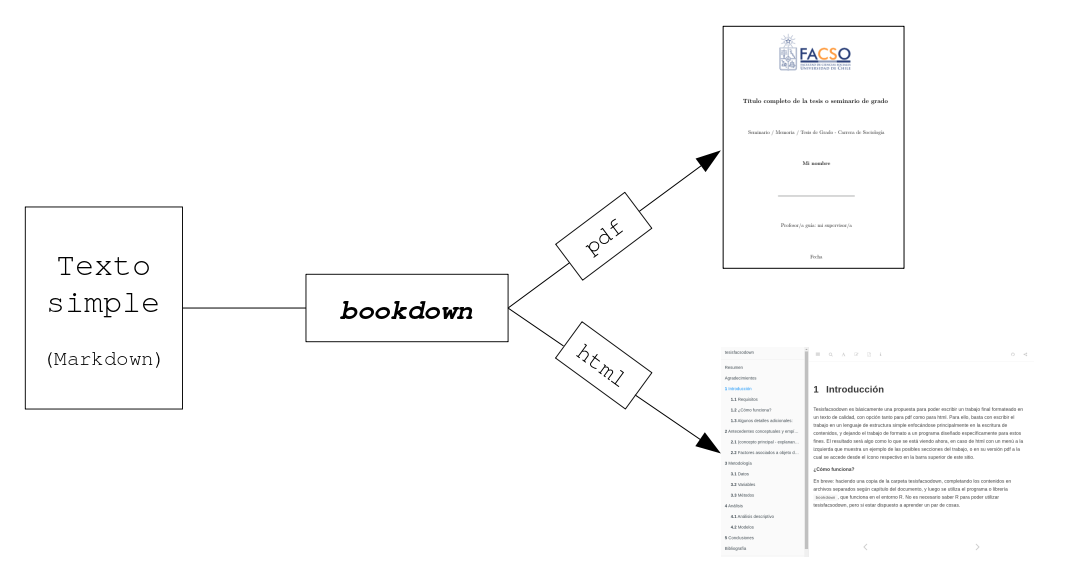
\includegraphics[width=1\linewidth]{images/flujobookdown} 

}

\caption{Flujo tesisfacsodown}\label{fig:flujo}
\end{figure}

Junto con realizar el trabajo de formato, quienes realizan análisis de datos con R tienen la posibilidad de incluir también los resultados (tablas, gráficos) de manera dinámica. Esto quiere decir que los análisis se realizan en el mismo documento, que se actualiza automáticamente en caso de modificaciones evitando así la ineficiencia de estar cortando y pegando cada vez que se realiza un cambio.

Tesisfacsodown está basada en otros proyectos similares como \href{https://github.com/ismayc/thesisdown}{\texttt{tesisdown}} y también \href{https://github.com/ulyngs/oxforddown}{\texttt{oxforddown}}.

\textbf{¿Cómo funciona?}

\emph{En breve}: haciendo una copia de la carpeta \emph{tesisfacsodown}, completando / reemplazando los contenidos en los archivos separados según secciones del documento (introducción, antecedentes, etc), y luego se utiliza el programa o librería \texttt{bookdown}, que funciona en el entorno R y que produce los documentos formateados en pdf y/o html. No es necesario saber R para poder utilizar tesisfacsodown, pero si estar dispuesto a aprender un par de cosas.

\hypertarget{requisitos}{%
\section{Requisitos}\label{requisitos}}

\begin{itemize}
\item
  Software: R/RStudio (ambos gratuitos).
\item
  librerías de R: \texttt{bookdown}, se instala desde RStudio en el menú Tools \textgreater{} Install packages \textgreater{} bookdown. Si se maneja R es más directo ejecutar desde la consola \texttt{install.packages("bookdown")}
\item
  Escritura: conocimiento de \emph{Markdown}, que es básicamente escribir simplemente texto con muy pocas marcas de edición (como encabezados, cursivas, negritas). Estas marcas de edición luego son interpretadas para poder generar documentos formateados en pdf, html (web) y también word. No requiere gran conocimiento previo, una introducción breve se puede encontrar \href{https://juancarloscastillo.github.io/in-socabi/lenguaje-reproducible.html}{aquí}.
\item
  No se requiere conocimiento de análisis de datos con R. Si bien este formato facilita la inclusión de resultados de análisis cuantitativos, puede ser perfectamente usado para trabajos con otras metodologías.
\item
  Si además de pdf se quiere publicar en formato web (es opcional) se necesitan conocimientos básicos de Git y Github. Una breve introducción se puede ver \href{https://cienciasocialabierta.netlify.app/class/08-class/}{aquí}, y con mucho mayor detalle en \url{https://happygitwithr.com/}.
\end{itemize}

\hypertarget{pasos}{%
\section{Pasos}\label{pasos}}

El primer paso consiste es obtener la carpeta de ejemplo \textbf{tesisfacsodown}, luego reemplazar algunos contenidos y obtener el documento formateado mediante un simple click en RStudio. Existen dos formas:

\begin{itemize}
\tightlist
\item
  simplemente bajar la carpeta desde \href{}{aquí}
\item
  para quienes tengan una cuenta en Github, lo más facil es hacer un fork del repositorio \url{https://github.com/juancarloscastillo/tesisfacsodown}, luego clonarlo localmente y comenzar a trabajar desde ahí. Esta opción es la más convieniente si se quiere luego publicar la tesis online (detalles abajo en sección de publicación web).
\end{itemize}

Una vez que se tiene la carpeta localmente, hacer doble click en el archivo \texttt{tesis.Rproj}, con lo que se abrirá RStudio (tiene que estar instalado previamente, tutorial \href{https://multivariada.netlify.app/class/\#installR}{aquí}). En RStudio hacer click sobre el botón ``build book'':

\begin{figure}

{\centering 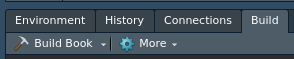
\includegraphics[width=0.6\linewidth]{images/build_book} 

}

\caption{Generando los documentos en pdf y html}\label{fig:build}
\end{figure}

Con esto aparecerá en el visor de RStudio (pestaña Viewer) el documento en formato (html) y también se generará el documento tesis.pdf en la carpeta docs, y al que se puede acceder desde el ícono pdf en la barra superior del documento en html. Lo que aparece en los documentos html y pdf es este mismo documento pdf/html que están viendo ahora, pero que ahora se encuentra guardado localmente en sus computadores y que pueden modificar con los contenidos de sus trabajos.

\emph{Detalles}

La carpeta tiene una serie de archivos y subcarpetas. Lo que hace el botón ``build book'' es activar la función \texttt{bookdown} de R que permite convertir el contenido escrito en Markdown hacia html y pdf. Para ello, los contenidos de la carpeta se organizan de la siguiente manera:

\begin{itemize}
\tightlist
\item
  \textbf{Archivo index.Rmd}: este archivo contiene

  \begin{itemize}
  \tightlist
  \item
    una serie de campos para poder personalizar e identificar la tesis, como título, autor, etc.
  \item
    de manera opcional se puede incluir un archivo con referencias bibliográficas .bib en caso de utilizar formato \texttt{bibtex} (que puede ser generado con gestores de referencias como Zotero o Mendeley, mayores detalles revisar \href{https://cienciasocialabierta.netlify.app/class/05-class/}{aquí}.
  \item
    también aparecen algunas opciones que tienen que ver con la generación del documento pdf y del sitio que no hay que modificar.
  \item
    finalmente, en este archivo también se puede incluir el Resumen / abstract del trabajo.
  \end{itemize}
\item
  \textbf{Secciones del trabajo}: es una propuesta de archivos markdown con extensión .Rmd que comienzan con un número, y es donde se separan las distintas secciones o capítulos. Podría también ser un solo gran archivo con todos los contenidos, pero esta división permite un mayor orden en el trabajo y también separa en distintas páginas web en el caso de publicación en este formato. El orden en que aparecen las secciones en el documento final se indica con un número al inicio del archivo (ej: 01-intro.Rmd). Los archivos de las secciones que aparecen en esta carpeta son solo de ejemplo y pueden ser eliminados / reemplazados de acuerdo a la estructura preferida.
\end{itemize}

Adicionalmente se encuentran:

\begin{itemize}
\item
  \emph{Archivos Readme} (.md y .html): contienen la información que aparece aquí, pueden ser eliminados posteriormente.
\item
  \emph{Archivos .yml}: son \_output y \_bookdown, y contienen información para generar los documentos pdf y html, no modificar
\item
  \emph{tesis.Rproj}: este es archivo que permite acceder a RStudio desde esta carpeta y activar las funciones necesarias para generar el documento formateado. Por lo tanto, luego de bajar la carpeta hacer doble click en este archivo.
\item
  \emph{tesis.bib}: es el archivo que contiene las referencias bibliográficas en formato bibtex, en caso de utilizar esta forma de referenciar. El archivo debe mantenerse con este nombre, de lo contrario no funcionará en el pdf.
\item
  \emph{Carpetas}:

  \begin{itemize}
  \tightlist
  \item
    images: para guardar imágenes que luego se puedan llamar desde los documentos. Para poder insertarlas desde los documentos Rmd se requiere dar la ruta a la imagen, por ejemplo: images/mi\_imagen.jpg. Que las imágenes se encuentren en esta carpeta es opcional, solo ayuda al orden de los documentos.
  \item
    templates: aquí se encuentran archivos que permiten dar formato a los documentos pdf y html (no modificar ni eliminar)
  \item
    docs: carpeta producida automáticamente que contiene los documentos generados y formateados en pdf y/o html.
  \end{itemize}
\end{itemize}

\hypertarget{algunos-detalles-adicionales}{%
\section{Algunos detalles adicionales:}\label{algunos-detalles-adicionales}}

\begin{itemize}
\item
  para más opciones de bookdown y detalles en general consultar \url{https://rubenfcasal.github.io/bookdown_intro/} (en español).
\item
  el formato del pdf es para ser impreso por los dos lados, por eso incluye algunas páginas en blanco (por ejemplo, la paǵina de atrás de la portada), y también los números de página se van alternando entre izquierda y derecha
\item
  Es posible generar una referenciación automática de tablas, imágenes y gráficos; además, se generan los índices respectivos en el formato pdf. Si estos provienen simplemente de archivos externos, se pueden almacenar en la carpeta ``imágenes'' e insertar así:
\end{itemize}

\begin{verbatim}
```{r nombre, echo=FALSE, fig.cap="Imagen de ejemplo", fig.align = 'center', out.width = '50%'}
knitr::include_graphics(path = "images/build_book.png")
```
\end{verbatim}

Lo que hay aquí es un trozo o ``chunk'' de código R, que en (R)Markdown se inserta simplemente entre tres acentos invertidos (`````''). Luego hay dos partes: las especificaciones de formato que van entre llaves \{\}, y la instrucción de lo que hay que hacer, en este caso llamar una imagen. Vamos por parte:

\begin{itemize}
\tightlist
\item
  especificaciones de formato:

  \begin{itemize}
  \tightlist
  \item
    \texttt{r} solamente informa que viene código R
  \item
    \texttt{nombre}: es el nombre que identifica al chunk, puede ser cualquiera
  \item
    \texttt{echo=FALSE}: esto se utiliza para que solo se muestre el resultado sin el código. Si fuera \texttt{TRUE}, entonces aparecería la función que llama la imagen además que la mi\_imagen
  \item
    \texttt{fig.cap}: el título de la imagen
  \item
    \texttt{fig.align}: alineación de la figura
  \item
    \texttt{out.width}: ancho en relación a la página. Hay diferentes formas de especificar las dimensiones, la ventaja de esta es que funciona bien tanto para pdf como para html, por lo que se recomienda
  \end{itemize}
\item
  instrucción o función: aquí se da la ruta a la imagen dentro del paréntesis con \texttt{path=}, y lo que antecede es la función para incluir gráficos de la librería knitr de R. Pero en simple: solo reemplazar el nombre de la imagen
\end{itemize}

Al incluir este trozo de código el resultado será el siguiente:

\begin{figure}

{\centering 
\includegraphics[width=0.5\linewidth]{images/facso} 

}

\caption{Imagen de ejemplo}\label{fig:nombre2}
\end{figure}

Donde la referenciación (caption) tiene el número 1.2, que quiere decir que es la segunda imagen del capítulo 1. En el pdf ahora esta figura aparece en el índice de figuras.

\begin{itemize}
\tightlist
\item
  en el caso de gráficos generados por R, también se insertan dentro de un chunk, por ejemplo
\end{itemize}

\begin{verbatim}
```{r echo=FALSE, fig.cap="Gráfico de ejemplo", fig.align = 'center', out.width = '50%'}
boxplot(Sepal.Length~Species,data=iris,
        xlab="Species", ylab="Sepal Length", main="Iris Boxplot")
```
\end{verbatim}

Y el resultado es este:

\begin{figure}

{\centering 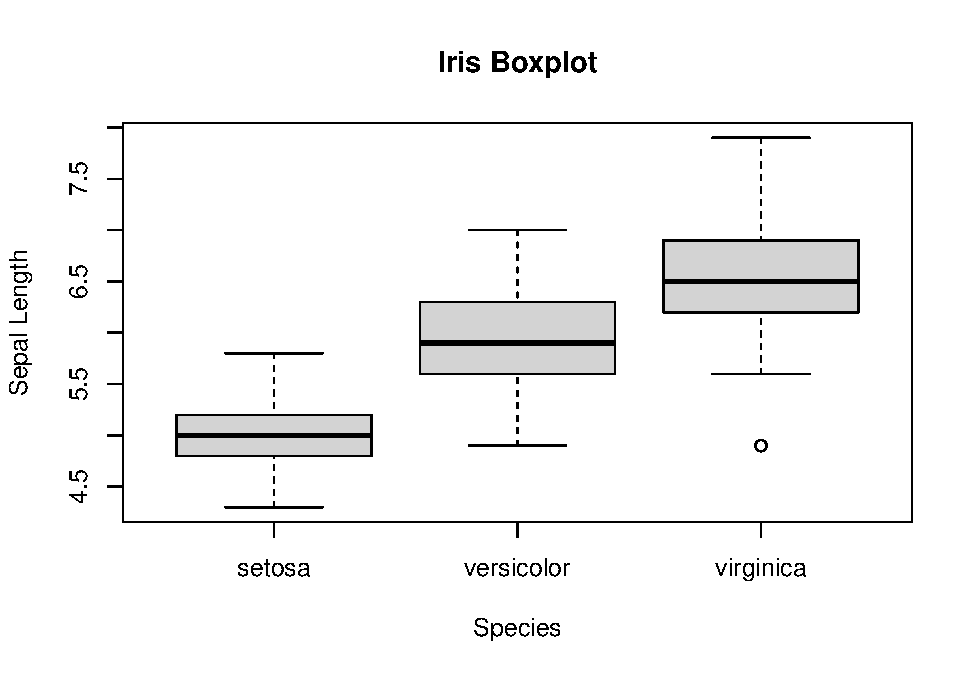
\includegraphics[width=0.5\linewidth]{tesis_files/figure-latex/unnamed-chunk-1-1} 

}

\caption{Gráfico de ejemplo}\label{fig:unnamed-chunk-1}
\end{figure}

\begin{itemize}
\tightlist
\item
  finalmente para las tablas producidas por R, es un poco más difícil si se quiere obtener el documento tanto en html como en pdf (que se genera vía Latex). En este caso, las tablas deben ser producidas en formato markdown, lo que no es muy común todavía en las distintas librerías de R que en genera privilegian o html o latex. La función para producir tablas markdown en R es principalmente \texttt{kable}, de la librería \texttt{knitr}, por ejemplo:
\end{itemize}

\begin{verbatim}
```{r tabla, echo=FALSE, caption="tabla de ejemplo", align = 'center'}
knitr::kable(head(iris), caption = "An example table caption.")
```
\end{verbatim}

\begin{Shaded}
\begin{Highlighting}[]
\NormalTok{knitr}\OperatorTok{::}\KeywordTok{kable}\NormalTok{(}\KeywordTok{head}\NormalTok{(iris), }\DataTypeTok{caption =} \StringTok{"Un ejemplo de tabla"}\NormalTok{)}
\end{Highlighting}
\end{Shaded}

\begin{table}

\caption{\label{tab:unnamed-chunk-2}Un ejemplo de tabla}
\centering
\begin{tabular}[t]{r|r|r|r|l}
\hline
Sepal.Length & Sepal.Width & Petal.Length & Petal.Width & Species\\
\hline
5.1 & 3.5 & 1.4 & 0.2 & setosa\\
\hline
4.9 & 3.0 & 1.4 & 0.2 & setosa\\
\hline
4.7 & 3.2 & 1.3 & 0.2 & setosa\\
\hline
4.6 & 3.1 & 1.5 & 0.2 & setosa\\
\hline
5.0 & 3.6 & 1.4 & 0.2 & setosa\\
\hline
5.4 & 3.9 & 1.7 & 0.4 & setosa\\
\hline
\end{tabular}
\end{table}

\begin{itemize}
\tightlist
\item
  nota sobre ubicación de imágenes y tablas en documento pdf (latex): en general se producen problemas en la ubicación, ya que automáticamente se ajustan al lugar disponible más cercano, sea atrás o delante. Si se quiere fijar la posición en el pdf, agregar antes y después del texto \texttt{\textbackslash{}FloarBarrier}, que es un comando latex que no será visible ni en pdf ni en html.
\end{itemize}

\hypertarget{publicaciuxf3n-web-y-versionamiento}{%
\section{Publicación web y versionamiento}\label{publicaciuxf3n-web-y-versionamiento}}

Una de las ventajas del formato html es poder publicarlo en línea para una fácil lectura y seguimiento. Esto puede ocurrir desde las fases iniciales o para el documento final, aumentando las posibilidades de difusión, colaboración y también de obtener revisiones y comentarios. De todas maneras, requiere algunos conocimientos más específicos que se introducen aquí.

Existen diferentes maneras de generar un sitio web con el documento, pero el más directo es a través de \textbf{Github} y de su opción \emph{githubpages}. Git/Github es una plataforma de versionamiento y colaboración cuyos detalles y posibilidades claramente no alcanzan a ser cubiertos en este espacio, pero si se desea mayor información se puede revisar \href{https://cienciasocialabierta.netlify.app/class/08-class/}{aquí}.

\begin{enumerate}
\def\labelenumi{\arabic{enumi}.}
\item
  Generación de repositorio: para quienes obtuvieron la carpeta partiendo desde Github con un \emph{fork / clone} de tesisfacsodown el repositorio se encuentra listo. En caso de haber bajado/copiado la carpeta manera simple, entonces a) crear un repositorio en Github, b) clonarlo localmente, c) copiar/mover los archivos de la carpeta tesisfacsodown a la carpeta clonada
\item
  Subir los cambios al repositorio (push)
\item
  Una vez que los archivos ya están en el repositorio Github ir a Settings \textgreater{} Github Pages y dejar de la siguiente manera:
\end{enumerate}

\begin{figure}

{\centering 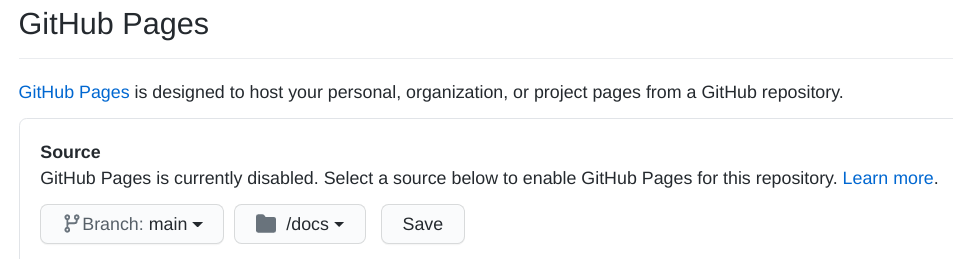
\includegraphics[width=0.6\linewidth]{images/githubpages} 

}

\caption{Bookdown en Github Pages}\label{fig:githubpages}
\end{figure}

Luego ``Save'' y se actualiza la página. Al bajar nuevamente a la sección de Github Pages debería aparecer ``Your site is ready to be published at {[}dirección web{]}''. Esa dirección es donde se puede acceder al sitio una vez que pasen algunos minutos.

\hypertarget{antecedentes-conceptuales-y-empuxedricos}{%
\chapter{Antecedentes conceptuales y empíricos}\label{antecedentes-conceptuales-y-empuxedricos}}

\hypertarget{concepto-principal---explanandum---objeto-de-estudio}{%
\section{(concepto principal - explanandum - objeto de estudio)}\label{concepto-principal---explanandum---objeto-de-estudio}}

\ldots{}

\hypertarget{factores-asociados-a-objeto-de-estudio}{%
\section{Factores asociados a objeto de estudio}\label{factores-asociados-a-objeto-de-estudio}}

\hypertarget{factor-1}{%
\subsection{Factor 1}\label{factor-1}}

Al final de esta sección, enunciar la hipótesis correspondiente

\hypertarget{factor-n}{%
\subsection{Factor N}\label{factor-n}}

Al final de esta sección, enunciar la hipótesis correspondiente

\hypertarget{metodologuxeda}{%
\chapter{Metodología}\label{metodologuxeda}}

\hypertarget{datos}{%
\section{Datos}\label{datos}}

\hypertarget{variables}{%
\section{Variables}\label{variables}}

\hypertarget{muxe9todos}{%
\section{Métodos}\label{muxe9todos}}

\hypertarget{anuxe1lisis}{%
\chapter{Análisis}\label{anuxe1lisis}}

\hypertarget{anuxe1lisis-descriptivo}{%
\section{Análisis descriptivo}\label{anuxe1lisis-descriptivo}}

\hypertarget{modelos}{%
\section{Modelos}\label{modelos}}

\hypertarget{conclusiones}{%
\chapter{Conclusiones}\label{conclusiones}}

\hypertarget{bibliografuxeda}{%
\chapter*{Bibliografía}\label{bibliografuxeda}}
\addcontentsline{toc}{chapter}{Bibliografía}

% %%%%%%%%%%%%%%%%%%%%%%%%%%%%%%%%%%%%%%%%%%%%%%%%%
% %%% Bibliography                              %%%
% %%%%%%%%%%%%%%%%%%%%%%%%%%%%%%%%%%%%%%%%%%%%%%%%%
% \addtocontents{toc}{\vspace{.5\baselineskip}}
% \cleardoublepage
% \phantomsection
% \addcontentsline{toc}{chapter}{\protect\numberline{}{Bibliography}}
\bibliography{tesis}

%% All books from our library (SfS) are already in a BiBTeX file
%% (Assbib). You can use Assbib combined with your personal BiBTeX file:
%% \bibliography{Myreferences,Assbib}. Of course, this will only work on
%% the computers at SfS, unless you copy the Assbib file
%%  --> /u/sfs/bib/Assbib.bib



\end{document}
